% Se pre-carga la información del estudiante sólo para poder emplear el macro de
% selección de versión (digital o impresa)
% ===============================================================================
% El estudiante debe llenar sus datos en esta sección para que la plantilla los 
% auto-importe y genere automáticamente las páginas de portada y de firmas 
% autorizadas.
% ===============================================================================
% Datos del estudiante:
% -------------------------------------------------------------------------------
% Nombre completo
\def \nombreestudiante {Jorge Antonio Lorenzana Ramos}
% Carné
\def \uvgcarne {17302}
% Facultad
\def \uvgfacultad {Ingeniería}
% Carrera
\def \uvgcarrera {Ingeniería Mecatrónica}

% Datos del trabajo:
% -------------------------------------------------------------------------------
% Título completo
\def \titulotesis {Implementación de un sistema de visión por computadora para el reconocimiento facial y de emociones para el rostro animatrónico de la Universidad del Valle de Guatemala}
% Año de entrega
\def \anoentrega {2021}
% Asesor
\def \nombreasesor {Ing. Kurt Kellner}

% Datos del tribunal examinador:
% -------------------------------------------------------------------------------
% Nombre del primer examinador
\def \nombreprimerex {MSc. Carlos Esquit}
% Nombre del segundo examinador
\def \nombresegundoex {Ing. Luis Pedro Montenegro}
% Año de aprobación
\def \anoaprobacion {2018}
% Mes de aprobación
\def \mesaprobacion {diciembre }
% Día de aprobación
\def \diaaprobacion {5 }

% Capítulos pre-definidos
% -------------------------------------------------------------------------------
% Comentar las líneas de las secciones que desean omitirse, por defecto se 
% se incluyen todas.
\def \CAPprefacio {Prefacio}
\def \CAPantecedentes {Antecedentes}
\def \CAPalcance {Alcance}
\def \CAPanexos {Anexos}
\def \CAPglosario {Glosario}

% Formato y estilo de la plantilla
% -------------------------------------------------------------------------------
% Modo impresión: Puede des-comentar la siguiente línea para generar un documento pdf sin la portada, para cuando se desee imprimir el documento para encuadernación
\def \printver {Versión del documento para impresión}

% Portada: Puede cambiarse la imagen en la portada al cambiar el nombre del 
% archivo siguiente. NOTA: debe tener la suficiente resolución para cubrir el área
% designada
\def \imagenportada {plantilla/portadacit.jpg}

% Referencias: Puede des-comentar la siguiente línea para utilizar el formato de referencias APA
%\def \usarAPA {Usar formato APA}

% Párrafo: Puede comentar la siguiente línea si desea emplear un formato de 
% párrafo distinto al establecido por defecto
\def \parpordefecto {Formato de párrafo por defecto}

% Capítulos y secciones: Puede des-comentar la siguiente línea para establecer el
% formato de los capítulos y secciones bajo el estándar original de UVG para
% trabajos de graduación. Este incluye: capítulos con numeración romana, secciones
% con letras mayúsculas, sub-secciones con números y sub-sub-secciones con letras
% minúsculas
%\def \capsecuvg {Formato UVG para capítulos y secciones}

\ifdefined\printver
    \documentclass[11pt, letterpaper, twoside, openright]{report}
\else
    \documentclass[11pt, letterpaper]{report}
\fi

% Eliminar la opción de twoside y openright si se desea generar la versión
% digital del documento en lugar de la versión impresa
%\documentclass[11pt, letterpaper, twoside, openright]{report}
\usepackage[spanish, es-nodecimaldot, es-noquoting]{babel}
% cambiar a spanish, mexico si se quiere emplear tabla en lugar de cuadro
\selectlanguage{spanish}
\usepackage[utf8]{inputenc}
\usepackage[T1]{fontenc}

\title{Plantilla para Trabajos de Graduación IE-MT 2019v4}
\author{MSc. Miguel Zea}
\date{\today}

% Información del estudiante en el archivo datos_estudiante.tex
% ===============================================================================
% El estudiante debe llenar sus datos en esta sección para que la plantilla los 
% auto-importe y genere automáticamente las páginas de portada y de firmas 
% autorizadas.
% ===============================================================================
% Datos del estudiante:
% -------------------------------------------------------------------------------
% Nombre completo
\def \nombreestudiante {Jorge Antonio Lorenzana Ramos}
% Carné
\def \uvgcarne {17302}
% Facultad
\def \uvgfacultad {Ingeniería}
% Carrera
\def \uvgcarrera {Ingeniería Mecatrónica}

% Datos del trabajo:
% -------------------------------------------------------------------------------
% Título completo
\def \titulotesis {Implementación de un sistema de visión por computadora para el reconocimiento facial y de emociones para el rostro animatrónico de la Universidad del Valle de Guatemala}
% Año de entrega
\def \anoentrega {2021}
% Asesor
\def \nombreasesor {Ing. Kurt Kellner}

% Datos del tribunal examinador:
% -------------------------------------------------------------------------------
% Nombre del primer examinador
\def \nombreprimerex {MSc. Carlos Esquit}
% Nombre del segundo examinador
\def \nombresegundoex {Ing. Luis Pedro Montenegro}
% Año de aprobación
\def \anoaprobacion {2018}
% Mes de aprobación
\def \mesaprobacion {diciembre }
% Día de aprobación
\def \diaaprobacion {5 }

% Capítulos pre-definidos
% -------------------------------------------------------------------------------
% Comentar las líneas de las secciones que desean omitirse, por defecto se 
% se incluyen todas.
\def \CAPprefacio {Prefacio}
\def \CAPantecedentes {Antecedentes}
\def \CAPalcance {Alcance}
\def \CAPanexos {Anexos}
\def \CAPglosario {Glosario}

% Formato y estilo de la plantilla
% -------------------------------------------------------------------------------
% Modo impresión: Puede des-comentar la siguiente línea para generar un documento pdf sin la portada, para cuando se desee imprimir el documento para encuadernación
\def \printver {Versión del documento para impresión}

% Portada: Puede cambiarse la imagen en la portada al cambiar el nombre del 
% archivo siguiente. NOTA: debe tener la suficiente resolución para cubrir el área
% designada
\def \imagenportada {plantilla/portadacit.jpg}

% Referencias: Puede des-comentar la siguiente línea para utilizar el formato de referencias APA
%\def \usarAPA {Usar formato APA}

% Párrafo: Puede comentar la siguiente línea si desea emplear un formato de 
% párrafo distinto al establecido por defecto
\def \parpordefecto {Formato de párrafo por defecto}

% Capítulos y secciones: Puede des-comentar la siguiente línea para establecer el
% formato de los capítulos y secciones bajo el estándar original de UVG para
% trabajos de graduación. Este incluye: capítulos con numeración romana, secciones
% con letras mayúsculas, sub-secciones con números y sub-sub-secciones con letras
% minúsculas
%\def \capsecuvg {Formato UVG para capítulos y secciones}
% ================================================================================
% En este archivo se colocan opciones adicionales para modificar el formato de la
% plantilla, para emplearse en otros tipos de documentos que no sean trabajos de
% graduación. Si usted está trabajando su tesis, NO modifique este archivo
% ================================================================================
% Capítulos pre-definidos
% --------------------------------------------------------------------------------
% Comentar las líneas de las secciones que desean omitirse, por defecto se 
% se incluyen todas.
\def \CAPportada {Portada}
\def \CAPcaratula {Caratula}
\def \CAPfirmas {Hoja de firmas}
\def \CAPindice {Índice general}
\def \CAPfiguras {Listado de figuras}
\def \CAPcuadros {Listado de cuadros}
\def \CAPresumen {Resumen}
\def \CAPabstract {Resumen}
\def \CAPintroduccion {Introducción}
\def \CAPobjetivos {Objetivos}
\def \CAPjustificacion {Justificación}
\def \CAPmarcoteorico {Marco teórico}
\def \CAPconclusiones {Conclusiones}
\def \CAPrecomendaciones {Recomendaciones}
\def \CAPbibliografia {Bibliografía}

% ==============================================================================
% DEFINICIÓN DE PAQUETES
% ==============================================================================
\usepackage{xcolor}
\usepackage{amsfonts}
\usepackage{amsmath}
\usepackage{amssymb}
\usepackage{amsthm}
\usepackage{amsfonts}
\usepackage{mathtools}
\usepackage{graphicx}
\usepackage{xfrac}
\usepackage{float}
\usepackage{mathtools}
\usepackage[hypertexnames=false]{hyperref}
% \usepackage{bookmark}
\usepackage[font=small]{caption}
\usepackage{subcaption}
%\usepackage{csquotes}
\usepackage{xpatch}
\usepackage{emptypage}
\usepackage{hyphenat}
\usepackage{fancyhdr}
\usepackage[backend=biber, style=ieee]{biblatex}
\ifdefined\usarAPA 
    \usepackage[backend=biber, style=apa]{biblatex}
\fi
\addbibresource{m-bibliografia.bib}

\usepackage[percent]{overpic}

\usepackage{chngcntr}

\ifdefined\CAPglosario
	%\usepackage[toc]{glossaries}
	\usepackage[numberedsection]{glossaries}
	\makeglossaries
    \newglossaryentry{latex}
{
    name=latex,
    description={Es un lenguaje de marcado adecuado especialmente para la creación de documentos científicos}
} 
 
\newglossaryentry{formula}
{
    name=fórmula,
    description={Una expresión matemática} 
}
\fi

% ==============================================================================
% MÁRGENES Y FORMATO GENERALES
% ==============================================================================
\usepackage[top=1in, left=1.5in, right=1in, bottom=1in]{geometry}
%Options: Sonny, Lenny, Glenn, Conny, Rejne, Bjarne, Bjornstrup
\usepackage[Sonny]{fncychap}

% ==============================================================================
% DEFINICIONES DE LA PLANTILLA
% ==============================================================================
\graphicspath{ {figuras/} }
\definecolor{uvg-green}{RGB}{17,71,52}
\newcommand{\defaultparformat}[1]{
	{\setlength{\parskip}{2ex}
     \input{#1}}
}
\ifdefined\capsecuvg
	\renewcommand\thechapter{\Roman{chapter}}
    \renewcommand\thesection{\Alph{section}}
	\renewcommand\thesubsection{\arabic{subsection}}
    \renewcommand\thesubsubsection{\alph{subsubection}}
\fi
\counterwithout{figure}{chapter}
\counterwithout{table}{chapter}
\counterwithout{equation}{chapter}

\newcommand{\blankpage}{
\newpage
\thispagestyle{empty}
\mbox{}
\newpage
}
% ==============================================================================

% Comandos definidos por el usuario en el archivo comandos_usuario.tex
\input{2-paquetes_y_comandos_usuario}

% ==============================================================================
% CUERPO DEL TRABAJO
% ==============================================================================
\pagestyle{headings}
\begin{document}

% ==============================================================================
% PORTADA
% ==============================================================================
\ifdefined\printver
    \let\CAPportada\undefined
\fi 

\ifdefined\CAPportada
    \cleardoublepage\phantomsection
    % \pdfbookmark{Portada}{toc}
	\newgeometry{left=3cm, bottom=0in, top=1in, right=3cm}
	\pagecolor{uvg-green}
	\thispagestyle{empty}

	\color{white}
	\noindent \hrulefill \par
	\vspace{0.1in}
	\noindent \Huge \nohyphens{\titulotesis} \par
	\noindent \hrulefill \par
	\noindent
	\LARGE \nombreestudiante

	\begin{figure}[b!]
    	%\makebox[\textwidth]{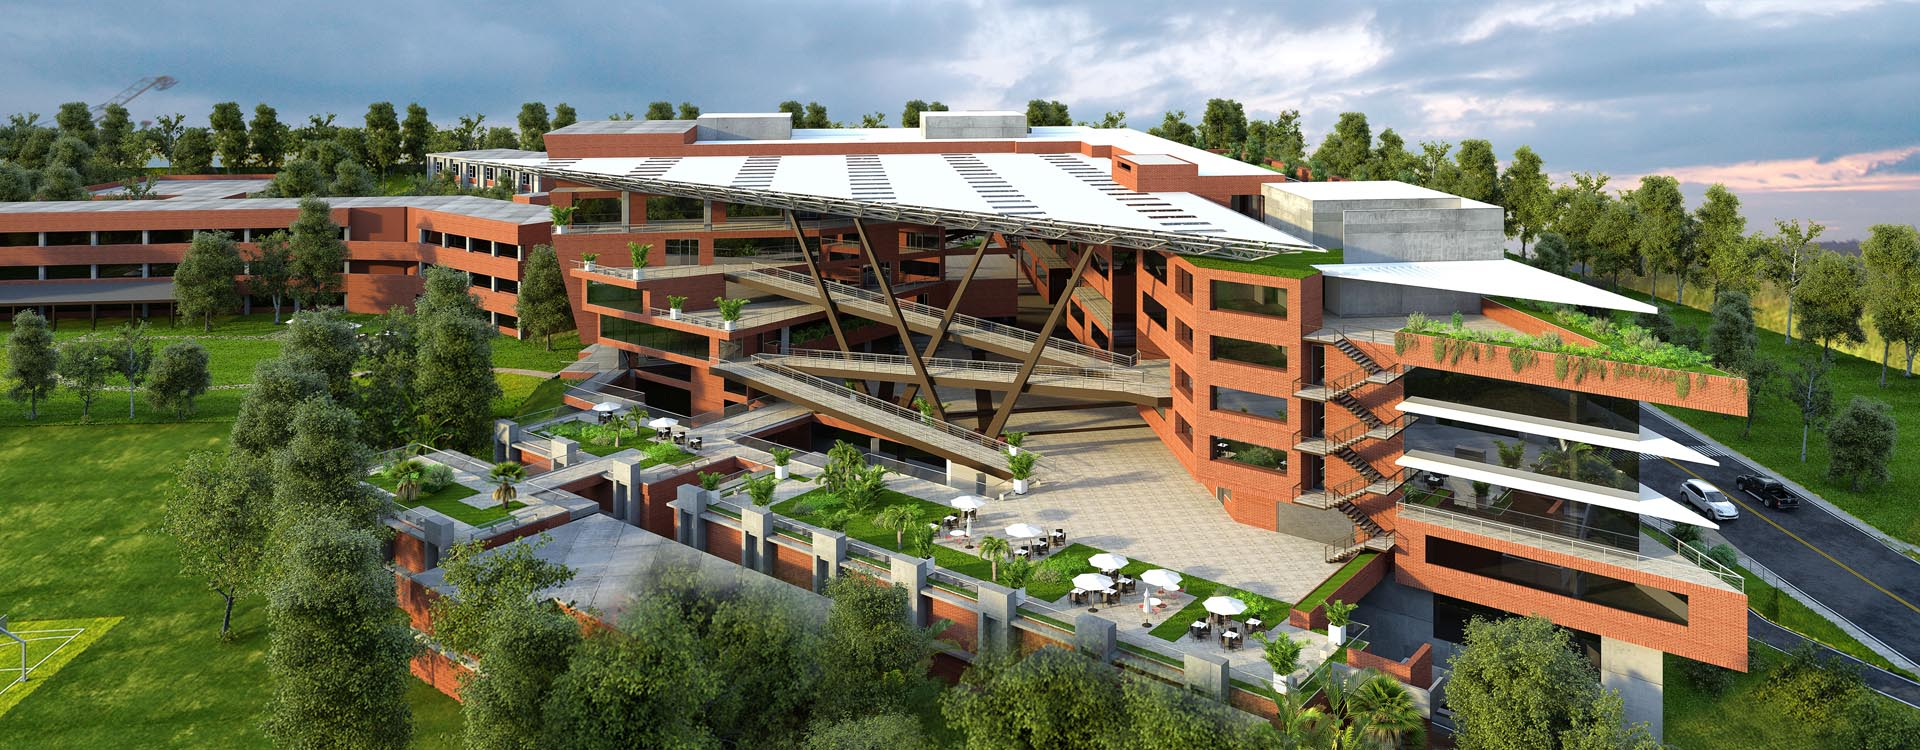
\includegraphics[height=13.25cm]{plantilla/portadacit.jpg}}
    	\makebox[\textwidth]{
    		\begin{overpic}[height=13.25cm]{\imagenportada}
     		\put(63,0){
\includegraphics[height=1.15in]{plantilla/fondologo_grande.png}}  
  			\put(64.5,2){
\includegraphics[height=0.55in]{plantilla/logoUVGblanco.eps}} 
        	\end{overpic}
    	}
    	%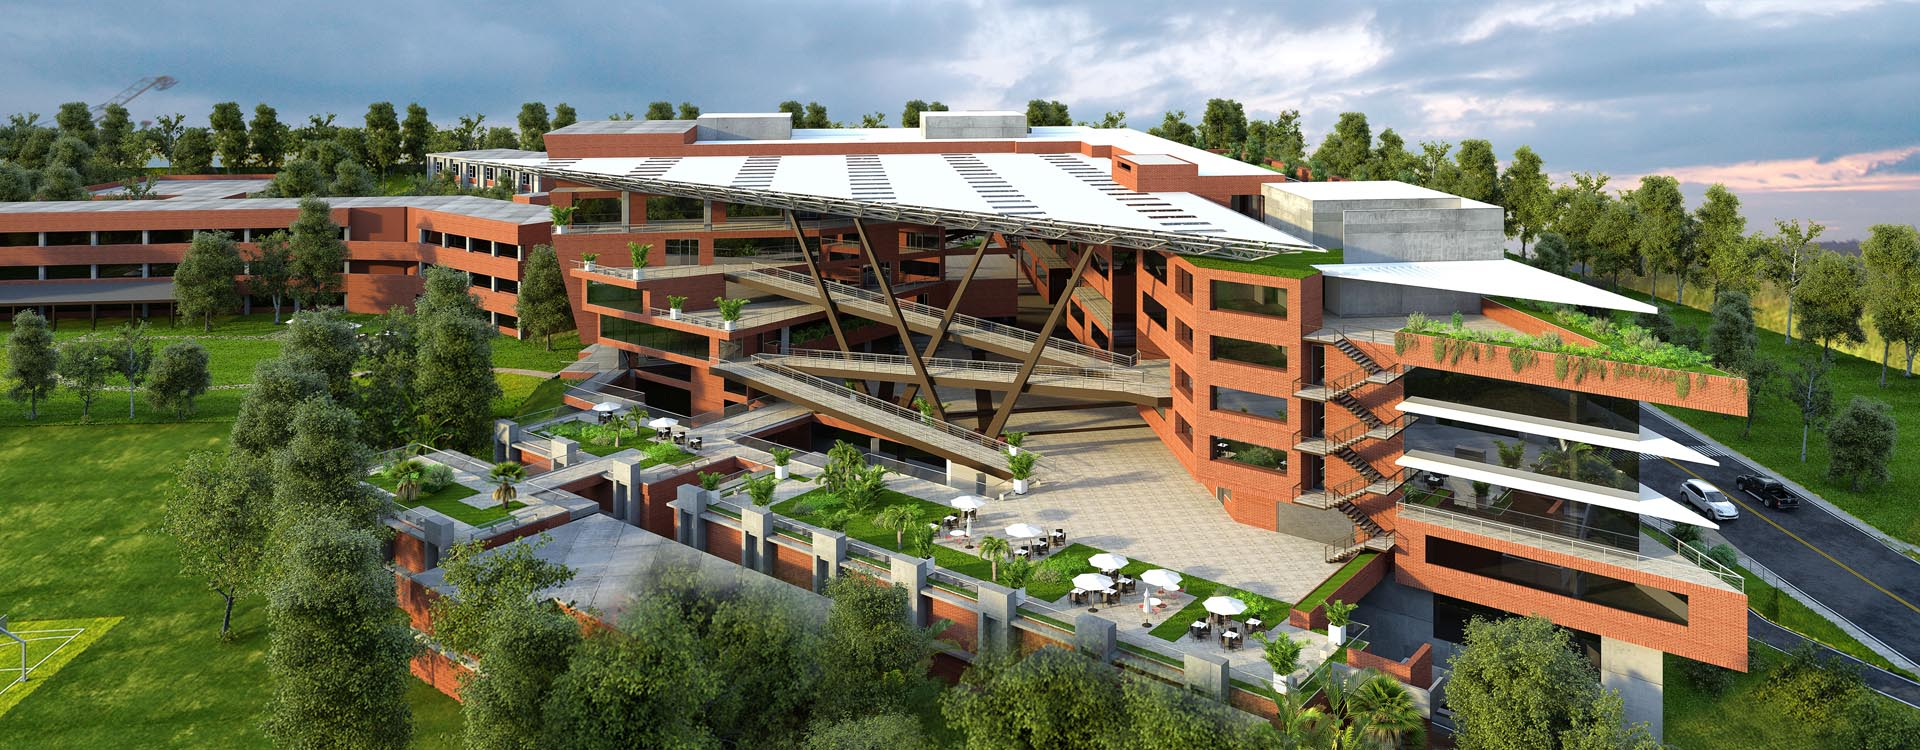
\includegraphics[height=13.25cm]{plantilla/portadacit.jpg}
	\end{figure}
	\restoregeometry
\fi

% ==============================================================================
% PRIMERAS PÁGINAS (Carátulas más hojas de guarda)
% ==============================================================================
\ifdefined\CAPcaratula
	\newpage
    \cleardoublepage\phantomsection
    % \pdfbookmark{Carátula}{toc}
	\pagecolor{white}
	\color{black}
	\setcounter{page}{1}
	\pagenumbering{roman}
	\thispagestyle{empty}
	\begin{center}
		\LARGE UNIVERSIDAD DEL VALLE DE GUATEMALA\\
		\LARGE Facultad de \uvgfacultad \\[0.75cm]
	\end{center}
	\begin{figure}[h]
		\begin{center}
		
\includegraphics[height=5.5 cm]{plantilla/escudoUVGnegro.eps}
		\vspace{0.5in}
		\end{center}
	\end{figure}
	\begin{center}
		\Large \textbf{\nohyphens{\titulotesis}} \\
		%\LARGE \textbf{\titulotesis} \\
		\vfill
		\Large \nohyphens{Trabajo de graduación presentado por \nombreestudiante \ para optar al grado académico de Licenciado en \uvgcarrera} \\
		\vfill
		\large Guatemala, \\
		\vspace{1em}
		\anoentrega
	\end{center}
    
    \ifdefined\printver	
	    \blankpage
	    \blankpage
	    
	    \newpage
	    \cleardoublepage\phantomsection
	    \pagecolor{white}
    	\color{black}
    	\setcounter{page}{1}
    	\pagenumbering{roman}
    	\thispagestyle{empty}
    	\begin{center}
    		\LARGE UNIVERSIDAD DEL VALLE DE GUATEMALA\\
    		\LARGE Facultad de \uvgfacultad \\[0.75cm]
    	\end{center}
    	\begin{figure}[h]
    		\begin{center}
    		
\includegraphics[height=5.5 cm]{plantilla/escudoUVGnegro.eps}
    		\vspace{0.5in}
    		\end{center}
    	\end{figure}
    	\begin{center}
    		\Large \textbf{\nohyphens{\titulotesis}} \\
    		%\LARGE \textbf{\titulotesis} \\
    		\vfill
    		\Large \nohyphens{Trabajo de graduación presentado por \nombreestudiante \ para optar al grado académico de Licenciado en \uvgcarrera} \\
    		\vfill
    		\large Guatemala, \\
    		\vspace{1em}
    		\anoentrega
    	\end{center}
    \fi
\fi

% ==============================================================================
% HOJA DE FIRMAS
% ==============================================================================
\ifdefined\CAPfirmas
	\newpage
	\cleardoublepage\phantomsection
	\thispagestyle{empty}
	\vspace*{0.5in}
	\large Vo.Bo.:\\[1cm]
	\begin{center}
		(f) \rule[1pt]{4 in}{1pt}\\
		\nombreasesor
	\end{center}
	\vspace{1in}

	Tribunal Examinador:\\[1cm]
	\begin{center}
		(f) \rule[1pt]{4 in}{1pt}\\
		\nombreasesor \\[1in]
		(f) \rule[1pt]{4 in}{1pt}\\
		\nombreprimerex \\[1in]
		(f) \rule[1pt]{4 in}{1pt}\\
		\nombresegundoex
	\end{center}
	\vspace{1in}

%	Fecha de aprobación: Guatemala, \rule[1pt]{0.5 in}{1pt} de \rule[1pt]{1 in}{1pt} de \anoaprobacion.
    Fecha de aprobación: Guatemala, \diaaprobacion de \mesaprobacion de \anoaprobacion.
	\normalsize
\fi

% Comentar para formato estilo libro en la numeración de páginas (NO 
% compatible con la guía UVG 2019)
\pagestyle{plain}
% ==============================================================================
% CONTENIDO DEL TRABAJO
% ==============================================================================
% PREFACIO
% ------------------------------------------------------------------------------
\ifdefined\CAPprefacio
	\newpage
	\cleardoublepage\phantomsection
    \chapter*{Prefacio}
    \ifdefined\parpordefecto
    	\defaultparformat{a-prefacio}
    \else
    	Lorem ipsum dolor sit amet, consectetur adipiscing elit. Cras vitae eleifend ipsum, ut mattis nunc. Pellentesque ac hendrerit lacus. Cras sollicitudin eget sem nec luctus. Vivamus aliquet lorem id elit venenatis pellentesque. Nam id orci iaculis, rutrum ipsum vel, porttitor magna. Etiam molestie vel elit sed suscipit. Proin dui risus, scelerisque porttitor cursus ac, tempor eget turpis. Aliquam ultricies congue ligula ac ornare. Duis id purus eu ex pharetra feugiat. Vivamus ac orci arcu. Nulla id diam quis erat rhoncus hendrerit. Class aptent taciti sociosqu ad litora torquent per conubia nostra, per inceptos himenaeos. Sed vulputate, metus vel efficitur fringilla, orci ex ultricies augue, sit amet rhoncus ex purus ut massa. Nam pharetra ipsum consequat est blandit, sed commodo nunc scelerisque. Maecenas ut suscipit libero. Sed vel euismod tellus.

Proin elit tellus, finibus et metus et, vestibulum ullamcorper est. Nulla viverra nisl id libero sodales, a porttitor est congue. Maecenas semper, felis ut rhoncus cursus, leo magna convallis ligula, at vehicula neque quam at ipsum. Integer commodo mattis eros sit amet tristique. Cras eu maximus arcu. Morbi condimentum dignissim enim non hendrerit. Sed molestie erat sit amet porttitor sagittis. Maecenas porttitor tincidunt erat, ac lacinia lacus sodales faucibus. Integer nec laoreet massa. Proin a arcu lorem. Donec at tincidunt arcu, et sodales neque. Morbi rhoncus, ligula porta lobortis faucibus, magna diam aliquet felis, nec ultrices metus turpis et libero. Integer efficitur erat dolor, quis iaculis metus dignissim eu.
    \fi
    \addcontentsline{toc}{chapter}{Prefacio}
\fi

% ÍNDICE GENERAL
% ------------------------------------------------------------------------------
\ifdefined\CAPindice
	\newpage
    \cleardoublepage\phantomsection
	\renewcommand{\contentsname}{Índice}
    %\phantomsection
    \pdfbookmark{\contentsname}{toc}
    %\pdfbookmark{Índice}{toc}
	\tableofcontents
\fi

% LISTADO DE FIGURAS
% ------------------------------------------------------------------------------
\ifdefined\CAPfiguras
	\newpage
    \cleardoublepage\phantomsection
	\renewcommand{\listfigurename}{Lista de figuras}
	\listoffigures
	\addcontentsline{toc}{chapter}{Lista de figuras}
\fi

% LISTADO DE CUADROS
% ------------------------------------------------------------------------------
\ifdefined\CAPcuadros
	\newpage
    \cleardoublepage\phantomsection
	\renewcommand{\listtablename}{Lista de cuadros}
	\listoftables
	\addcontentsline{toc}{chapter}{Lista de cuadros}
\fi

% RESUMEN
% ------------------------------------------------------------------------------
\ifdefined\CAPresumen
	\newpage
    \cleardoublepage\phantomsection
	\chapter*{Resumen}
	\ifdefined\parpordefecto
		\defaultparformat{b-resumen}
	\else
		La animatrónica es el proceso de fabricación y programación de mecanismos robóticos que son capaces de replicar el movimiento y comportamiento de seres vivos. En este proyecto se replica el movimiento de una cabeza humana y el comportamiento antes las emociones de otro ser humano. Anteriormente se había trabajado el modelo 3D del rostro animatrónico, con un alto parecido a la anatomía humana y este es capaz de realizar movimientos bastante allegados a la realidad de un rostro. 

Actualmente se trabaja en el comportamiento del mismo, con el objetivo de que pueda detectar el rostro de otra persona y reconocer las emociones que este presenta. Por ello se necesita crear un software que permita capturar imágenes en tiempo real y analizarlas de la misma manera para obtener información relevante que luego será procesada, por una red neuronal, para dar una respuesta estimulante para el usuario. Además de sincronizar los movimientos del rostro con la respuesta que se está dando para así poder replicar el comportamiento deseado.

El detector de emociones consta de dos etapas, la creación del modelo y la implementación del mismo. Se busca crear un modelo que reconozca las siete emociones básicas del ser humano y que está sea la raíz para poder desarrollar las respuestas del robot. Estas respuestas se procesarán en una red neuronal que puede modificarse o ampliarse en el futuro, para que este proyecto se pueda continuar trabajando y pueda aprovecharse, no solo para la Universidad del Valle de Guatemala, sino también para otras instituciones.
	\fi
	\addcontentsline{toc}{chapter}{Resumen}
\fi

% ABSTRACT
% ------------------------------------------------------------------------------
\ifdefined\CAPabstract
	\newpage
    \cleardoublepage\phantomsection
	\chapter*{Abstract}
	\ifdefined\parpordefecto
		\defaultparformat{c-abstract}
	\else
		This is an abstract of the study developed under the
	\fi
	\addcontentsline{toc}{chapter}{Abstract}
\fi

% INTRODUCCIÓN
% ------------------------------------------------------------------------------
\ifdefined\CAPintroduccion
	\newpage
	\cleardoublepage
	\pagenumbering{arabic}
	\setcounter{page}{1}
	\chapter{Introducción}
	\ifdefined\parpordefecto
		\defaultparformat{d-introduccion}
	\else
		Lorem ipsum dolor sit amet, consectetur adipiscing elit. Quisque eget consequat risus. Praesent a quam lacinia, consequat eros id, auctor tellus. Phasellus a dapibus arcu, vitae luctus leo. Aliquam erat volutpat. Suspendisse ac velit quam. Nullam risus nibh, lobortis vehicula elit non, pellentesque volutpat odio. Donec feugiat porta sapien gravida interdum. Cras odio nunc, lobortis sed pellentesque imperdiet, facilisis eu quam. Praesent pharetra, orci at tincidunt lacinia, neque nulla ornare lacus, ut malesuada elit risus non mi. Fusce pellentesque vitae sapien sed mollis. Curabitur viverra at nulla vitae porta. In et mauris lorem.

Vestibulum faucibus fringilla justo, eget facilisis elit convallis sit amet. Morbi nisi metus, hendrerit quis pellentesque non, faucibus at leo. Proin consectetur, est vel facilisis facilisis, arcu felis vestibulum quam, et fringilla metus neque at enim. Nunc justo mauris, egestas quis maximus eget, viverra vehicula nunc. Fusce eu nulla elementum, condimentum diam at, aliquam leo. Nullam sed sodales enim, eu imperdiet risus. Aliquam ornare augue leo, fringilla mattis nunc facilisis eget. Nam faucibus, libero a aliquet fermentum, magna arcu ultrices lacus, a placerat tortor turpis ut purus.

Integer eget ligula non metus egestas rutrum sit amet ut tellus. Aliquam vel convallis est, eu sodales leo. Proin consequat nisi at nunc malesuada gravida. Aliquam erat volutpat. Aliquam finibus interdum dignissim. Etiam feugiat hendrerit nisl, hendrerit feugiat ex malesuada in. Cras tempus eget arcu vitae congue. Ut non tristique mauris. Vivamus in mattis ipsum. Cras bibendum, enim bibendum commodo accumsan, ligula nulla porttitor ex, et pharetra eros nisl eget ex. Morbi at semper arcu. Curabitur massa sem, maximus id metus ut, molestie tempus quam. Vivamus dictum nunc vitae elit malesuada convallis. Donec ac semper turpis, non scelerisque justo. In congue risus id vulputate gravida. Nam ut mattis sapien.
	\fi
\fi

% ANTECEDENTES
% ------------------------------------------------------------------------------
\ifdefined\CAPantecedentes
	\newpage
	\chapter{Antecedentes}
	\ifdefined\parpordefecto
    	\defaultparformat{e-antecedentes}
    \else
    	\subsection*{Sistema de detección de rostro y reconocimiento de gestos para robot animatrónico}
Anteriormente en la Universidad del Valle de Guatemala (UVG), el estudiante Luis Eduardo Ruano Argueta trabajó un software para la detección del rostro y emociones. Para este proyecto se utilizó Python, OpenCV, Base de datos de rostros, entre otros. Se utilizan dos algoritmos distintos para clasificar las distintas emociones y ellos utilizan una cámara Logitech 920 para obtener las imágenes en tiempo real \cite{Ruano2019Tesis}.

El objetivo principal de este proyecto es implementar por medio de software un programa que pueda darle seguimiento a los rostros y el reconocimiento de expresiones faciales de las personas. Para esto se realizó una comparación entre dos algoritmos. Uno que utiliza algoritmos en cascada y otro que utiliza las marcas de cara. Se analizaron ambos algoritmos en dos ambientes diferentes, uno controlado y uno no controlado para evaluar el desempeño de ambos en aspectos como la distancia máxima, movimientos laterales, agresividad de movimientos y rotación con respecto al ángulo de visión. Entre los resultados destaca el alcance máximo del algoritmo \textit{Haar cascade}, con un alcance máximo de 5.31m en ambientes controlados y abiertos. Mientras que el algoritmo de marcas de cara destaca en cuando a la detección cuando existe un ángulo de rotación mayor a 45°al ángulo de visión respecto a la cámara. \cite{Ruano2019Tesis}.

Los algoritmos seleccionados para el \textit{Haar cascade} y el algoritmo de marcas de cara son \textit{Fisher Face} y SVM respectivamente. Para el algoritmo \textit{Fisher Face} se realizó reconstrucción de imágenes y representación de estas por medio de dispersión de datos. Para el algoritmo SVM se utilizó marcas de cara para generar entrenamientos \cite{Ruano2019Tesis}.

Para las bases de datos se utilizó una base de datos descargada llamada \textit{Cohn-Kanade} y las bases generadas \textit{UVG}, \textit{UVG 2m}, \textit{Ambiente 2} y \textit{Personalizada}. Estas bases de datos se utilizaron para entrenar los algoritmos para trabajar en los distintos ambientes, ya sean controlados  o no, cantidad de iluminación, distancia, entre otros \cite{Ruano2019Tesis}.

Se tuvieron problemas al momento de reconocer ciertas expresiones, ya que los algoritmos las confundian con otras. Al realizar las pruebas se limitó la cantidad de expresiones para detectar a 3: Feliz, enojo y sorpresa. Al realizar esta modificación se tuvo una mejora en los resultados teniendo un porcentaje de éxito por encima del 68\%, donde el más bajo fue de 68.21\% para el ambiente UVG 2m con el algoritmo \textit{Fisher Face} \cite{Ruano2019Tesis}.

\begin{figure}[h]
    \centering
    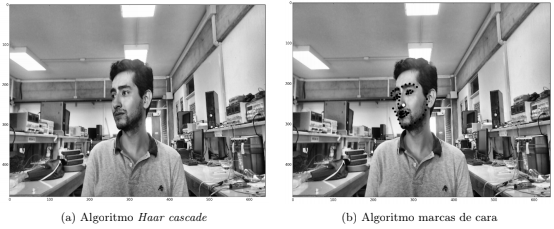
\includegraphics[width=0.7\textwidth]{figuras/Ruano_Result.png}
    \caption{Detección de rostros con angulo de visión de 45°. \cite{Ruano2019Tesis}}
    \label{fig:RuanoResult}
\end{figure}

\subsection*{Detector de emociones utilizando OpenCV}
El usuario de medium.com, Karan  Sethi, publicó un artículo donde presenta el procedimiento y resultados de la deteccion de sus rostro y el reconocimiento de 5 emociones. El usuario utilizó el software de OpenCV para la visión por computadora y Keras para el aprendizaje automático. El procedimiento que utilizó se reduce en dos grandes etapas, la creación del modelo, que incluye el entrenamiento del mismo, y la implementación del modelo para el reconocimiento de emociones en tiempo real \cite{Karan}.

En el artículo, Karan, dice explicitamente que los prerrequisitos para poder realizar este proyecto es tener conocimiento básico de los sigueintes temas:
\begin{itemize}
\item Python
\item OpenCV
\item Red neuronal de convolución (CNN)
\item numpy
\end{itemize}

El objetivo principal de Karan es crear una red neuronal de convolución utilizando Keras, la API para Python sobre (\textit{Deep Learning}), para detectar emociones en tiempo real a través de la realimentación al sistema de una cámara en tiempo real \cite{Karan}.

Para esto, él realiza la primera etapa, la creación del modelo, en cinco tareas. La primera tarea es importar todos los módulos necesarios en el proyecto, declarar algunas variables como la cantidad de emociones, los pixeles de las imágenes que se estarán utilizando y la cantidad de muestras que se tomarán antes de que el modelo se actualice. Seguido de eso, realiza la segunda tarea, la cual es importar el \textit{dataset} que se estará utilizando. Él utiliza el \textit{dataset} de \textbf{fer2013}, un \textit{dataset} de libre uso alojado en la plataforma de \textbf{kaggle}. Este contiene siete clases, las cuales corresponden a las siete emociones básicas, sin embargo, karan utiliza solo cinco de esas clases. Ahora continuamos con la tercera tarea la cual consiste en expandir el \textit{dataset} que se está utilizando de manera artificial. Para esto utiliza \textbf{Keras}, que tiene la capacidad de ajustar modelos usando la clase . Ahora, la cuarta tarea es crear el cerebro de nuestro modelo, es decir, la CNN. Se define el modelo que se estará utilizando que, en el caso de Karan, es el modelo secuencial que define que todas las capas en la red serán secuenciales y las alamcenará en una variable del modelo. Por último, la quinta tarea es compilar y entrenar el modelo. Para esto se importan algunas librerías, se crean algunas funciones y luego se compila y ajusta el modelo. Con esto ya solo quedaría implementar el modelo para el reconocmiento de emociones en tiempo real \cite{Karan}.

Ahora, Karan, realiza la segunda etapa. La cual consta de crear el driver para usar el modelo creado anteriormente. Lo primero es importar algunos módulos necesarios para el funcionamiento del código, como las herramientas de OpenCV. También hay que cargar el modelo y el algoritmo de clasificación, él utiliza \textbf{Haar Cascade} que es una algortimo para identificar objetos en imágenes o videos. Después de programar y terminar el código el detector de emociones estaría terminado. Y como resultado se tendría lo mostrado en la Figura \ref{fig:KaranResult} \cite{Karan}.

\begin{figure}[h]
    \centering
    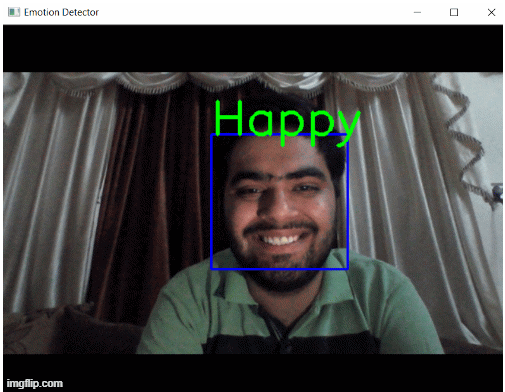
\includegraphics[width=0.5\textwidth]{figuras/Karan_Result.png}
    \caption{Resultado del detector de emociones de Karan Sethi. \cite{Karan}.}
    \label{fig:KaranResult}
\end{figure}
    \fi  
\fi

% JUSTIFICACIÓN
% ------------------------------------------------------------------------------
\ifdefined\CAPjustificacion
	\newpage
	\chapter{Justificación}
	\ifdefined\parpordefecto
		\defaultparformat{f-justificacion}
	\else
		El ámbito de la animatrónica en Guatemala es un ámbito que no está desarrollado. Siendo algo que se puede aplicar en varios campos de trabajo como lo es la industria del entretenimiento, el turismo o cualquiera que necesite de dar información. Si bien un animatrónico no puede sustituir por completo un recurso humano, si que puede ser de utilidad para cumplir ciertas funciones. Este rostro podrá ser utilizado en la Universidad del Valle de Guatemala para brindar al usuario información útil acerca de la misma, reaccionando al estado de ánimo. Así como está aplicación se puede aplicar en museos, para dar información acerca de las distintas piezas que se exponen. De esta manera ayudar a instituciones a darse a basto para cumplir con la demanda de información y evitar que el personal humano realice la misma actividad multiples veces. Además de empezar con el desarrollo y aprendizaje de creaciones de inteligencias pseudoartificiales.

El desarrollo de animatrónicos es un buen ejercicio para un ingeniero que busca especializarse en el campo de la robótica, automatización e incluso en el campo biomédico, ya que cuenta con replicar movimientos humanos y diseñar en base a la anatomía del ser humano. Es un proceso muy complejo que requiere de conocimientos de los distintos campos para llevarse a cabo. Por otro lado, el desarrollo del detector de emociones es un proceso que necesita de campos como programación y psicología, dos campos completamente distintos. Esto porque hay que realizar un software capaz de capturar imágenes y procesarlas, y hay que tener conocimientos en el área de psicología para poder interpretar la emoción que se está mostrando y como responder ante esa emoción. 

Así pues, el desarrollo de este proyecto es una oportunidad que abarca muchas áreas de aprendizaje y de desarrollo, tanto para las instituciones como para el país. Además de ser un proyecto que puede seguir creciendo con el tiempo, de manera que abre oportunidades para seguir aprendiendo e implementando nuevos sistemas, nuevas interacciones e incluso nuevas respuestas.
	\fi
\fi

% OBJETIVOS
% ------------------------------------------------------------------------------
\ifdefined\CAPobjetivos
	\newpage
	\chapter{Objetivos}
	\ifdefined\parpordefecto
		\defaultparformat{g-objetivos}
	\else
		\section{Objetivo General}
Desarrollar e implementar un sistema de visión por computador de reconocimiento facial y de emociones para la interacción con el rostro animatrónico de la Universidad del Valle de Guatemala

\section{Objetivos Específicos}
\begin{itemize}
\item Identificar, por medio de las herramientas de software seleccionadas, las siete emociones básicas: alegría, tristeza, miedo, enojo, asco, desprecio, sorpresa.
\item Implementar un sistema en el que el rostro animatrónico imite directamente los gestos de una persona.
\item Implementar un sistema de respuestas pre-programadas para interactuar con el usuario según la emoción que percibe el rostro animatrónico.
\item Implementar una interfaz gráfica de uso sencillo que sirva de puente entre el hardware y los sensores.
\item Desarrollar un árbol de decisiones para la continua interacción Humano-Robot.
\end{itemize}
	\fi
\fi

% ALCANCE
% ------------------------------------------------------------------------------
\ifdefined\CAPalcance
	\newpage
	\chapter{Alcance}
	\ifdefined\parpordefecto
    	\defaultparformat{h-alcance}
    \else
    	Podemos usar \Gls{latex} para escribir de forma ordenada una \gls{formula} matemática. 
    \fi 
\fi

% MARCO TEÓRICO
% ------------------------------------------------------------------------------
\ifdefined\CAPmarcoteorico
	\newpage
	\chapter{Marco teórico}
	\ifdefined\parpordefecto
		\defaultparformat{i-marco_teorico}
	\else
		\section*{Las 7 emociones básicas}
Las emociones evolucionaron para cumplir la función de promover la supervivencia física, pero el desarrollo de la cultura humana también ha impulsado la evolución de las emociones en el sentido de que esta
s cumplan funciones relativas a metas sociales, tales como llevarse bien con los demás y avanzar en la comunidad. Las emociones básicas tienen funciones sociales además de las de supervivencia \cite{rulicki2012cnv}.

Estas siete emociones básicas son:
\begin{itemize}
\item \textbf{Alegría:} Sensación dichosa de placer y bienestar \cite{rulicki2012cnv}.
\item \textbf{Tristeza:} Sensación opresiva de pérdida o carencia que produce desánimo \cite{rulicki2012cnv}.
\item \textbf{Miedo:} Sensación de agitación causada por una percepción de peligro debida a riesgos físicos, morales, o la presencia de dolor \cite{rulicki2012cnv}.
\item \textbf{Enojo:} Sensación perturbadora que resulta de una ofensa, una torpeza propia o un obstáculo natural. Generalmente incluye el deseo de reaccionar agresivamente \cite{rulicki2012cnv}.
\item \textbf{Asco:} Sensación de repugnancia debida a la percepción de un estímulo desagradable a los sentidos \cite{rulicki2012cnv}.
\item \textbf{Desprecio:} Sensación de rechazo o desestimación hacia otra persona o cosa, por considerarla inferior, indigna o carente de valor \cite{rulicki2012cnv}.
\item \textbf{Sorpresa:} Sensación súbita e inesperada de asombro \cite{rulicki2012cnv}.
\end{itemize}

\begin{figure}[h]
    \centering
    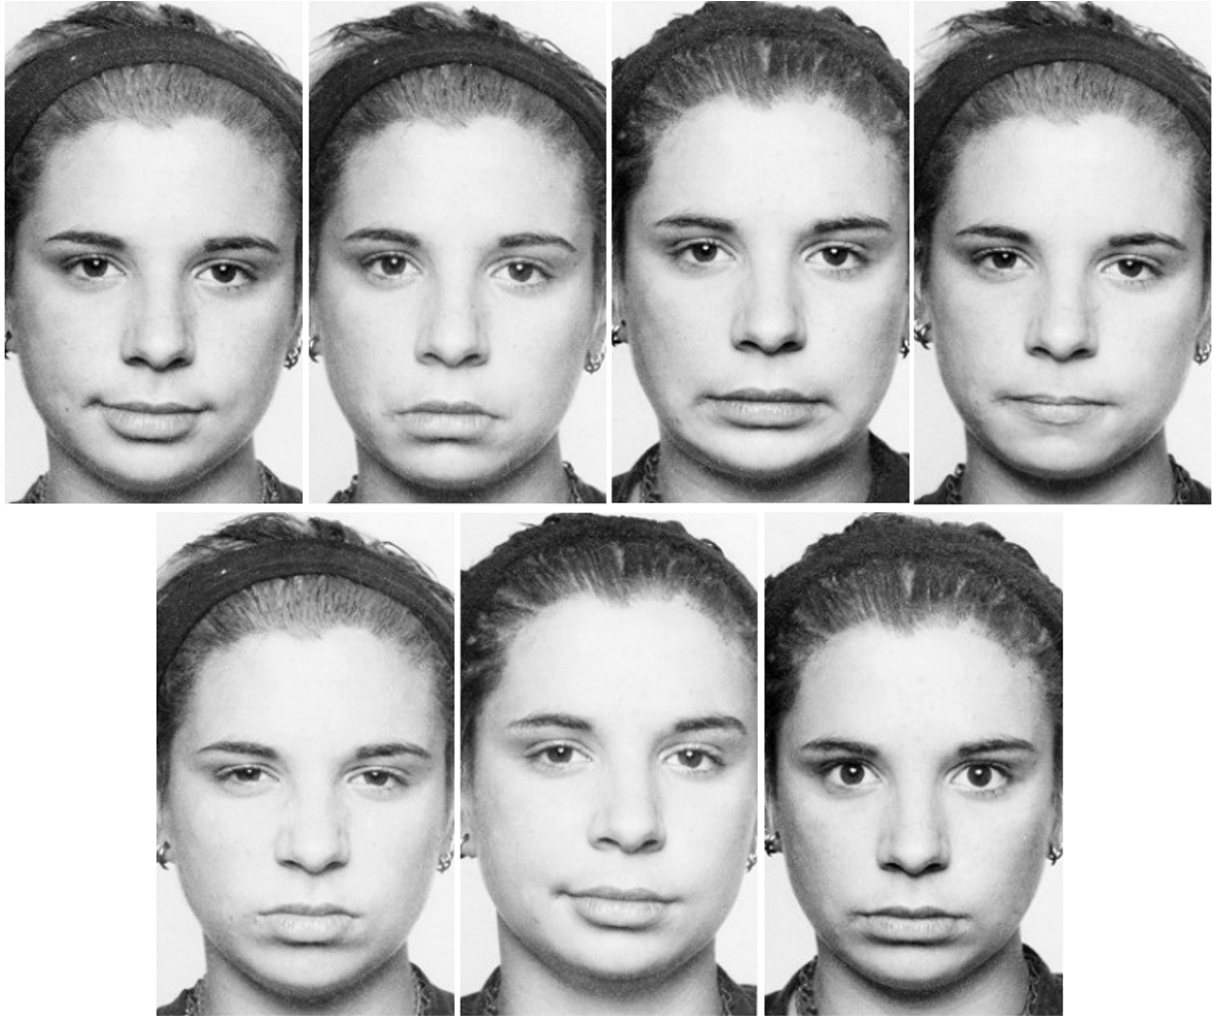
\includegraphics[width=0.6\textwidth]{Emociones.png}
    \caption{Gestos de distintas emociones \cite{ekman2017rostro}.}
    \label{fig:Emociones}
\end{figure}

\subsection*{Las señales faciales de las emociones}
Las señales faciales son las configuraciones de los distintos rasgos particulares de cada emoción, que son producidas por movimientos involuntarios en los músculos del rostro. Según Ekman, las expresiones de las emociones nos dan información acerca de lo que está ocurriendo dentro de la persona, lo que posiblemente ocurrió antes de que se desarrollara la emoción y aquello que puede llegar a pasar en consecuencia de la emoción. Para esto se utiliza el sistema FACS (Facial Action Coding System), que es un sistema de codificación que recoge todos movimientos expresivos del rostro en unidades de acción (AU) \cite{ekman2017rostro}.

\begin{table}[H]
\centering
\begin{tabular}{|c|c|}
\hline
\textbf{AU} & \textbf{Acción} \\ \hline
1             & Levantamiento interior de ceja      \\ \hline
2             & Levantamiento exterior de ceja      \\ \hline
4             & Bajar cejas                         \\ \hline
5             & Levantamiento del párpado superior  \\ \hline
6             & Levantamiento de mejillas           \\ \hline
7             & Apretar párpados                    \\ \hline
8             & Labios encimados uno de otro        \\ \hline
9             & Arrugar nariz                       \\ \hline
10            & Levantamiento del labio superior    \\ \hline
11            & Profundidad nasolabial              \\ \hline
12            & Tiramiento labial esquinal          \\ \hline
13            & Tiramiento labial frontal           \\ \hline
14            & Hoyuelo facial                      \\ \hline
15            & Depresión labial esquinal           \\ \hline
16            & Depresión labial frontal            \\ \hline
17            & Levantamiento de barbilla           \\ \hline
18            & Arruga labial                       \\ \hline
19            & Muestro de lengua                   \\ \hline
20            & Apretar los labios                  \\ \hline
21            & Apretamiento de cuello              \\ \hline
22            & Embudo labial                       \\ \hline
23            & Morder labios                       \\ \hline
24            & Presión labial                      \\ \hline
25            & Deslizamiento labial                \\ \hline
26            & Caída de la mandíbula               \\ \hline
27            & Apretamiento bucal                  \\ \hline
28            & Lamido labial                       \\ \hline
29            & Tracción de la mandíbula            \\ \hline
30            & Deslizamiento de mandíbula          \\ \hline
31            & Contracción mandibular              \\ \hline
32            & Mordida labial                      \\ \hline
33            & Succión de mejillas                 \\ \hline
34            & Inflar mejillas                     \\ \hline
35            & soplido de mejillas                 \\ \hline
36            & Protuberancia de lengua             \\ \hline
37            & Limpieza labial                     \\ \hline
38            & Dilatado nasal                      \\ \hline
39            & Compresión nasal                    \\ \hline
\end{tabular}
\caption{Lista de Unidades de acción y descripciones de acción.}
    \label{cuadro:AU}
\end{table}

\section*{Como reconocer las emociones en los demás}

\subsection*{Alegría}
El truco para reconocer correctamente la alegría está en los ojos. Concretamente, en las temidas patas de gallo. Si no aparecen estas características arrugas en el contorno exterior de los ojos, la sonrisa no se considera espontánea, sino una sonrisa social o intencionada. Los dos movimientos musculares o unidades de acción más características de la alegría son la elevación simétrica de las comisuras de los labios (AU12) y el ascenso de las mejillas (AU6) \cite{ReconocerLasEmociones}.

\begin{figure}[h]
    \centering
    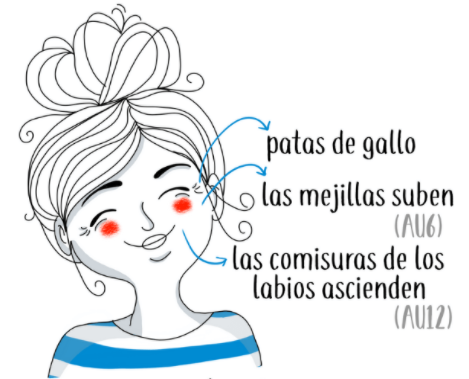
\includegraphics[width=0.25\textwidth]{Alegria.png}
    \caption{Rasgos de alegría \cite{ReconocerLasEmociones}.}
    \label{fig:Alegria}
\end{figure}

\subsection*{Sorpresa}
Las tres unidades de acción más características de la sorpresa son la elevación simétrica de las cejas hacia el exterior (AU2), la apertura desorbitada de los párpados (AU5) y la caída de la mandíbula (AU26). El truco para reconocer correctamente la sorpresa está en los ojos y en la mandíbula. Los ojos parecen desorbitar, por efecto de la subida de los párpados superiores. Y lo que es más curioso, queda al descubierto la parte blanca de la esclerótica por encima del iris, que normalmente no vemos \cite{ReconocerLasEmociones}.

\begin{figure}[h]
    \centering
    \includegraphics[width=0.25\textwidth]{sorpresa.png}
    \caption{Rasgos de sorpresa \cite{ReconocerLasEmociones}.}
    \label{fig:Sorpresa}
\end{figure}

\subsection*{Tristeza}
Las unidades de acción más características de la tristeza son la elevación de las cejas hacia el interior (AU1), la caída de las comisuras de los labios (AU15), y la subida del mentón (AU17). El truco para reconocer correctamente la tristeza está en el comportamiento de las cejas. Lo más habitual es que, al subir hacia el interior, la activación del músculo frontal forme unas arrugas horizontales en el centro de la frente \cite{ReconocerLasEmociones}.

\begin{figure}[h]
    \centering
    
\includegraphics[width=0.25\textwidth]{Tristeza.png}
    \caption{Rasgos de tristeza \cite{ReconocerLasEmociones}.}
    \label{fig:Tristeza}
\end{figure}

\subsection*{Miedo}
El truco para reconocer correctamente el miedo está en fijarnos bien en los ojos, y no confundirlos con los de la sorpresa. Las dos unidades de acción más características del miedo son la elevación de los párpados superiores (AU5), y la retracción o estiramiento horizontal de los labios (AU20) \cite{ReconocerLasEmociones}.

\begin{figure}[h]
    \centering
    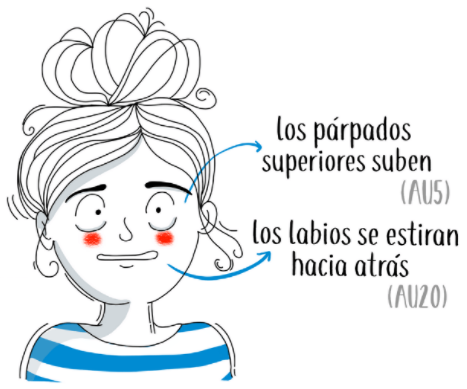
\includegraphics[width=0.25\textwidth]{Miedo.png}
    \caption{Rasgos de Miedo \cite{ReconocerLasEmociones}.}
    \label{fig:Miedo}
\end{figure}

\subsection*{Ira}
Las tres unidades de acción más características de la ira son juntar y bajar las cejas sobre la nariz (AU4), la tensión en los párpados inferiores (AU7) y la proyección de la mandíbula hacia adelante (AU29). El truco para reconocer correctamente la ira está en el ceño fruncido, formado por las típicas arrugas sobre la nariz al juntar y bajar las cejas \cite{ReconocerLasEmociones}.

\begin{figure}[h]
    \centering
    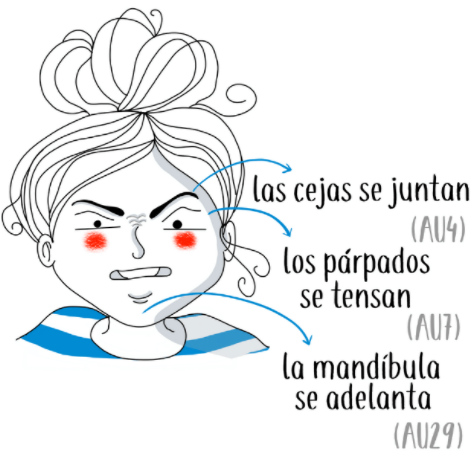
\includegraphics[width=0.25\textwidth]{Ira.png}
    \caption{Rasgos de ira \cite{ReconocerLasEmociones}.}
    \label{fig:Ira}
\end{figure}

\subsection*{Asco}
Las dos unidades de acción más características del asco son arrugar la nariz (AU9), y elevar el labio superior (AU10). El truco para reconocer correctamente el asco está en la activación del pliegue nasolabial, fácilmente reconocible porque el labio superior asciende y la nariz se arruga \cite{ReconocerLasEmociones}.

\begin{figure}[h]
    \centering
    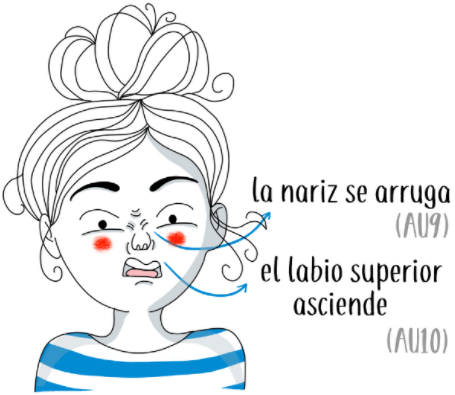
\includegraphics[width=0.25\textwidth]{Asco.png}
    \caption{Rasgos de asco \cite{ReconocerLasEmociones}.}
    \label{fig:Asco}
\end{figure}

\subsection*{Desprecio}
La única unidad de acción características del desprecio es la retracción de una de las comisuras de los labios hacia la mejilla (AU14), formando el típico hoyuelo en un solo lado de la cara, o acentuando su existencia.El truco para reconocer correctamente el desprecio está en el típico hoyuelo, formado en una sola de las mejillas cuando los labios se retraen hacia un lado de la cara. El problema está en que no siempre se aprecia con claridad, sobre todo si la microexpresión es leve y rápida \cite{ReconocerLasEmociones}.

\begin{figure}[h]
    \centering
    
\includegraphics[width=0.25\textwidth]{Desprecio.png}
    \caption{Rasgos de desprecio \cite{ReconocerLasEmociones}.}
    \label{fig:Desprecio}
\end{figure}

\section*{Visión por computadora}
\subsection*{OpenCV}
OpenCV es una biblioteca de software de visión por computadora y de aprendizaje automático (\textit{Machine learning}) de código abierto. OpenCv se creó para aplicaciones de visión por computadora y para acelerar el uso de la percepción de la máquina en productos comerciales. Al ser un producto con licencia BSD, facilita que las empresas utilicen y modifiquen el código. La biblioteca tiene más de 2500 algoritmos optimizados que incluyen un conjunto completo de algoritmos de aprendizaje automático y visión por computadora clásicos y de última generación. Estos algoritmos se pueden utilizar para detectar y reconocer rostros, identificar objetos, clasificar acciones humanas en videos, entre otros. OpenCV tiene más de 47 mil usuarios en la comunidad y un número estimado de descargas superior a 18 millones. La biblioteca se utiliza ampliamente en empresas, grupos de investigación y organismos gubernamentales. Tiene interfaces C ++, Python, Java y MATLAB y es compatible con Windows, Linux, Android y Mac OS \cite{OpenCV}.

\subsection*{SimpleCV}
SimpleCV es un marco de código abierto para crear aplicaciones de visión por computadora. Con él, obtiene acceso a varias bibliotecas de visión por computadora de alta potencia, como OpenCV, sin tener que aprender primero sobre profundidades de bits, formatos de archivo, espacios de color, administración de búfer, valores propios o almacenamiento de matriz versus mapa de bits. Esta es la visión por computadora simplificada \cite{SimpleCV}.

\subsection*{Accord.NET Framework}
Accord.NET Framework es un marco de aprendizaje automático .NET combinado con bibliotecas de procesamiento de audio e imagen completamente escritas en C\#. Es un marco completo para crear aplicaciones de visión por computadora, audición por computadora, procesamiento de señales y estadísticas, incluso para uso comercial. Un conjunto completo de aplicaciones que proporciona un comienzo rápido para comenzar a funcionar rápidamente, y una extensa documentación y wiki ayudan a completar los detalles \cite{Accord.NET}.

\subsection*{BoofCV}
BoofCV es una biblioteca de código abierto escrita desde cero para la visión por computadora en tiempo real. Su funcionalidad cubre una variedad de temas, procesamiento de imágenes de bajo nivel, calibración de la cámara, detección / seguimiento de funciones, estructura desde el movimiento, detección fiducial y reconocimiento. BoofCV ha sido lanzado bajo una licencia Apache 2.0 para uso académico y comercial \cite{BoofCV}.

\section*{Aprendizaje automático}
\subsection*{Keras}
Keras es una API de aprendizaje profundo escrita en Python, que se ejecuta sobre la plataforma de aprendizaje automático TensorFlow. Fue desarrollado con un enfoque en permitir una experimentación rápida. Ser capaz de pasar de la idea al resultado lo más rápido posible es clave para hacer una buena investigación. Ofrece APIs consistentes y simples, minimiza la cantidad de acciones del usuario necesarias para casos de uso comunes y proporciona mensajes de error claros y procesables. También cuenta con una extensa documentación y guías para desarrolladores \cite{Keras}.

\subsection*{TensorFlow}
TensorFlow es una plataforma de código abierto de extremo a extremo para el aprendizaje automático. Cuenta con un ecosistema integral y flexible de herramientas, bibliotecas y recursos de la comunidad que les permite a los investigadores innovar con el aprendizaje automático y, a los desarrolladores, compilar e implementar con facilidad aplicaciones con tecnología de AA. TensorFlow ofrece varios niveles de abstracción para que puedas elegir el que se adecue a tus necesidades. Compila y entrena modelos mediante la API de alto nivel de Keras, que ayuda a que los primeros pasos con TensorFlow y el aprendizaje automático sean sencillos \cite{TensorFlow}.

\subsection*{PyTorch}
Es un paquete de Python diseñado para realizar cálculos numéricos haciendo uso de la programación de tensores. Además permite su ejecución en GPU para acelerar los cálculos. Normalmente PyTorch es usado tanto para sustituir numpy y procesar los cálculos en GPU como para la investigación y desarrollo en el campo del machine learning, centrado principalmente en el desarrollo de redes neuronales. PyTorch es una librería muy reciente y pese a ello dispone de una gran cantidad de manuales y tutoriales donde encontrar ejemplos. Además de una comunidad que crece a pasos agigantados. PyTorch dispone una interfaz muy sencilla para la creación de redes neuronales pese a trabajar de forma directa con tensores sin la necesidad de una librería a un nivel superior como pueda ser Keras para Theano o Tensorflow \cite{PyTorch}.
	\fi
\fi

% CAPÍTULOS
% ------------------------------------------------------------------------------
\newpage
\ifdefined\parpordefecto
	\defaultparformat{j-capitulos}
\else
	\chapter{Modelo 3D}
Lo primero en realizar serán las modificaciones y arreglos al modelo mecánico del rostro animatrónico. Estas modificaciones incluyen la base del rostro animatrónico, por una que sea más resistente y más eficiente que la que se tiene actualmente. De esta manera se podrá probar el funcionamiento del mismo para saber que movimientos son posibles de realizar y así tener una idea de como tendrá que comportarse. Con las piezas diseñadas e impresas se procederá a desarmar el modelo y reemplazar todas las piezas defectuosas, esto incluye modelos 3D, tornillos, tuercas y todas las piezas mecánicas necesarias para la reconstrucción del rostro. Con el rostro reconstruido se pondrá a funcionar los servomotores para verificar que todo esté funcionando correctamente, que movimientos son capaces de realizar y si todos los componentes electrónicos están funcionando o si hay alguno que deba cambiarse.

\chapter{Modelo de reconocimiento}


\chapter{Detector de emociones}

\chapter{Respuesta a las emociones}

\chapter{GUI}
\fi

% CONCLUSIONES
% ------------------------------------------------------------------------------
\ifdefined\CAPconclusiones
	\newpage
	\chapter{Conclusiones}
	\ifdefined\parpordefecto
		\defaultparformat{k-conclusiones}
	\else
		\input{k-conclusiones}
	\fi
\fi

% RECOMENDACIONES
% ------------------------------------------------------------------------------
\ifdefined\CAPrecomendaciones
	\newpage
	\chapter{Recomendaciones}
	\ifdefined\parpordefecto
		\defaultparformat{l-recomendaciones}
	\else
		\input{l-recomendaciones}
	\fi
\fi

% BIBLIOGRAFÍA
% ------------------------------------------------------------------------------
\ifdefined\CAPbibliografia
	\newpage
    \cleardoublepage\phantomsection
	\chapter{\bibname}
    \printbibliography[heading=none]
\fi

% ANEXOS
% ------------------------------------------------------------------------------
\ifdefined\CAPanexos
	\newpage
	\chapter{Anexos}
	\ifdefined\parpordefecto
		\defaultparformat{n-anexos}
	\else
		\input{n-anexos}
	\fi
\fi

% GLOSARIO
% ------------------------------------------------------------------------------
\ifdefined\CAPglosario
	\newpage
	\printglossary
\fi

\end{document}